\documentclass{article}

\usepackage[hangul]{kotex}
\usepackage{amsmath}
\usepackage{tikz}
\usepackage{minted}
\usepackage{geometry}
\usepackage{enumitem}
\usepackage{multicol}
\usepackage[linguistics]{forest}
\usepackage{algorithm}
\usepackage{algpseudocode}
\usepackage{hyperref}

\hypersetup{
  colorlinks   = false, %Colours links instead of ugly boxes
  urlcolor     = blue, %Colour for external hyperlinks
  linkcolor    = black, %Colour of internal links
  citecolor   = red %Colour of citations
}

\geometry{
  a4paper,
  left=2.7cm,
  right=2.7cm,
  top=2.7cm,
  bottom=2.7cm,
}

\setmonohangulfont{D2Coding}

\title{프로그래밍과 문제해결 \\ Assignment \#2}
\author{무은재학부 박재원 (2024****)}
\date{\today}

\begin{document}

\begin{titlepage}
	\centering
	{\huge CSED101 프로그래밍과 문제해결\par}
	\vspace{0.5cm}
	{\LARGE Assignment \#2\par}
	\vspace{0.5cm}
	{\large \today\par}
	\vfill
  
  \begin{multicols}{2}
    \vphantom{}
    \columnbreak
  {
    \Large 
    \begin{description}[nosep, align=right, labelwidth=\widthof{00000000000000000}]
      \item[학과] 무은재학부
      \item[학번] 2024****
      \item[이름] 박재원
      \item[POVIS ID] ****
    \end{description}
  }
  \end{multicols}

  \vspace{1cm}


  \begin{quote}
    명예서약 (Honor code)

    ``나는 이 프로그래밍 과제를 다른 사람의 부적절한 도움 없이 완수하였습니다.''
  \end{quote}

\end{titlepage}

\tableofcontents

\section{개요}

본 과제는 성적 관리 CLI 프로그램을 만드는 것이다.
처음 실행 시 파일로부터 학생별 성적 데이터를 읽어오며,
이후 여러 명령어를 통해 조회, 생성, 수정, 삭제 등의 작업을 수행할 수 있다.
학생별 중간고사와 기말고사의 평균 성적 및 학점, 전체 학생들의 성적의 평균, 중앙값, 표준편차도 계산해준다.
이렇게 처리한 성적 정보는 프로그램 종료 시 파일로 다시 저장할 수 있다.

\section{설계}

\subsection{구조도}

프로그램의 전체 구조도는 그림 \ref{fig:structurechart}와 같다. 중요하지 않은 함수는 생략했다.

\begin{description}
  \item[입력부] 성적 파일 읽기, 명령어 입력, 각 명령별 세부 정보/옵션 입력 등
  \item[처리부] Raw 성적 데이터을 이차원 리스트로 변환, 평균 $\cdot$ 학점 등 계산, 정렬, 학번으로 학생 찾기, 각 명령어에 따른 작업 수행 등
  \item[출력부] 학생 목록 출력, 명령어 실행 결과 출력, 에러 메시지 출력 등
\end{description}

\begin{figure}
  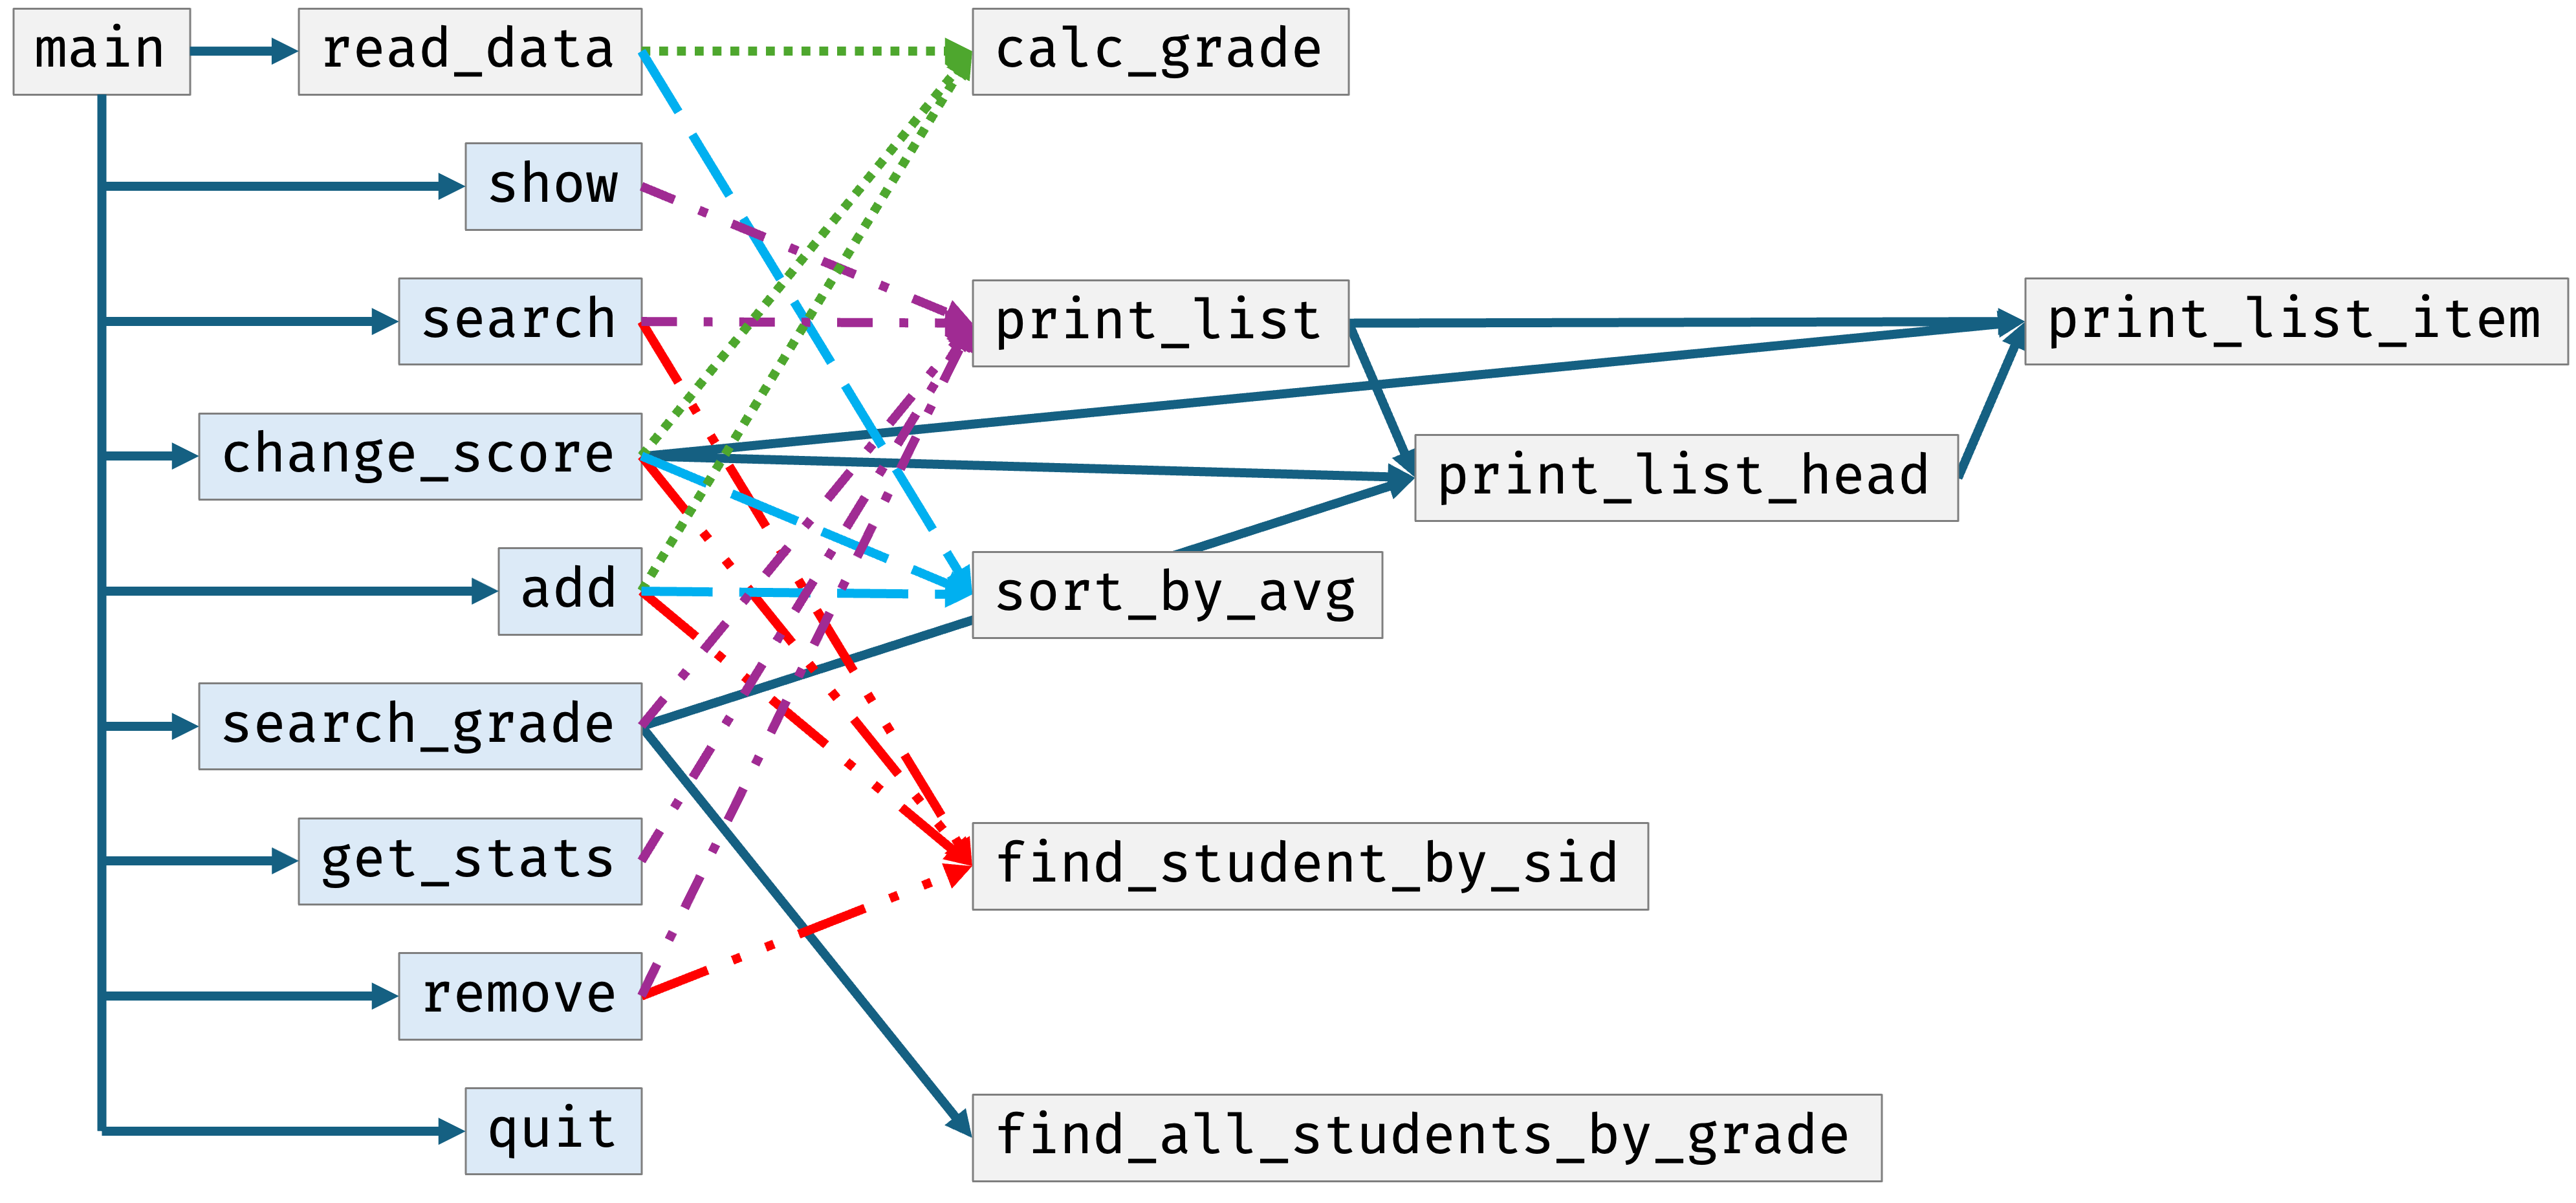
\includegraphics[width=\textwidth]{structurechart.png}
  \caption{본 프로그램의 전체 구조도}
  \label{fig:structurechart}
\end{figure}

\subsection{알고리즘}
프로그램의 알고리즘을 의사코드로 나타내면 알고리즘 \ref{alg:all}\과 같다.

\begin{algorithm}
  \caption{본 프로그램 주요 부분의 의사 코드} \label{alg:all}
  \begin{algorithmic}
    \State 학생데이터 $\gets$ 입력받은 파일명에 해당하는 파일의 내용
    \State 학생데이터 정렬 및 목록 출력
    \While {}
      \State 명령어 $\gets$ 사용자 입력
      \If {명령어 $=$ show}
        \State 학생데이터 목록 출력
      \ElsIf {명령어 $=$ search}
        \State 대상학번 $\gets$ 사용자 입력
        \State 학생 $\gets$ 학생데이터에서 대상학번에 해당하는 학생 찾기
        \State 학생 출력
      \ElsIf {명령어 $=$ changescore}
        \State 대상학번, 대상시험, 새\_점수 $\gets$ 사용자 입력
        \State 학생 $\gets$ 학생데이터에서 대상학번에 해당하는 학생 찾기
        \State 학생의 대상시험 점수를 새\_점수로 수정
        \State 학생 평균, 학점 계산 \& 학생데이터 정렬
        \State 학생 수정 전/후 출력
      \ElsIf {명령어 $=$ add}
        \State 학번, 이름, 중간점수, 기말점수 $\gets$ 사용자 입력
        \State 평균, 학점 $\gets$ 중간점수, 기말점수로부터 평균, 학점 계산
        \State 학생데이터에 정보 추가
      \ElsIf {명령어 $=$ searchgrade}
        \State 대상학점 $\gets$ 사용자 입력
        \State 대상학생들 $\gets$ 학생데이터에서 학점이 대상학점인 학생 찾기
        \State 대상학생들 목록 출력
      \ElsIf {명령어 $=$ getstats}
        \State 학생데이터의 중간점수, 기말점수, 평균점수에 대해 중앙값, 평균, 표준편차 계산
        \State 계산 결과 출력
      \ElsIf {명령어 $=$ remove}
        \State 대상학번 $\gets$ 사용자 입력
        \State 학생 $\gets$ 학생데이터에서 대상학번에 해당하는 학생 찾기
        \State 학생 출력
        \If {진짜 삭제할지 물어보고 yes라 답하면}
          \State 학생데이터에서 학생 삭제
        \EndIf
      \ElsIf {명령어 $=$ quit}
        \State 저장여부 $\gets$ 사용자 입력
        \If {저장여부 $=$ yes}
          \State 입력받은 파일명을 갖는 파일에 학생데이터 출력
        \EndIf
        \State while 문 break
      \EndIf
    \EndWhile
  \end{algorithmic}
\end{algorithm}

\section{실행 방법 및 예제}

본 과제는 MacOS\footnote{특정 OS에 종속적인 기능을 사용하지 않으므로 다른 운영체제에서도 정상 작동하리라 예상된다.}, CPython 3.12.2에서 작성 및 테스트되었다.

본 과제를 실행하려면 우선 다음과 같이 assn2.py와 students.txt(혹은 적절한 학생데이터 파일)를 같은 디렉토리에 위치시킨 후,
파이썬 코드를 실행시키면 된다. 프로그램이 실행되고 students.txt(혹은 원하는 학생데이터 파일의 이름)을 입력하면 해당 파일의 내용을 불러온다. 이후 원하는 명령어를 입력하여 프로그램을 사용할 수 있다.
\begin{minted}[]{bash}
  ls
  # assn2.py      students.txt
  python assn2.py
  # Input the score file name: _
  # ...
\end{minted}

실제 프로그램 실행 모습은 그림 \ref{img:1} $\sim$ \ref{img:9}와 같다.

\begin{figure}
  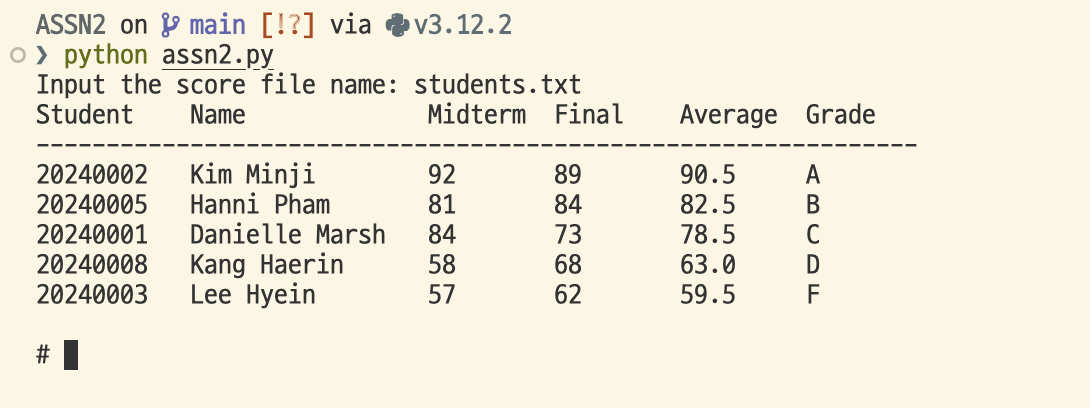
\includegraphics[width=\textwidth]{screenshots/1.png}
  \caption{실행 모습. 실행 직후}
  \label{img:1}
\end{figure}
\begin{figure}
  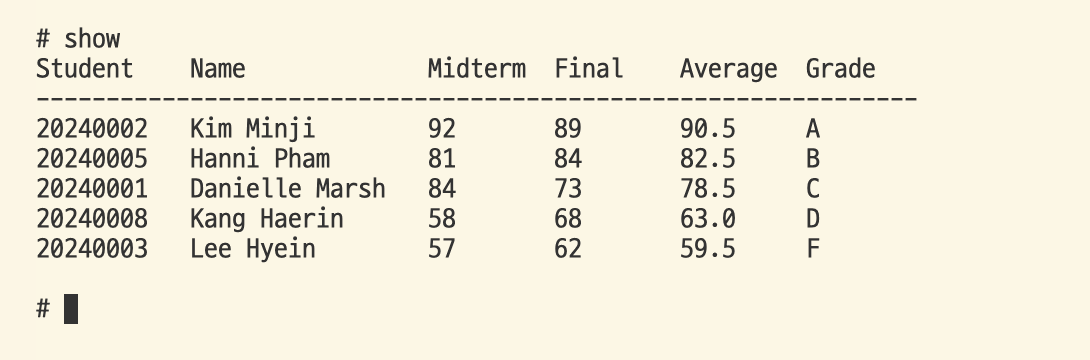
\includegraphics[width=\textwidth]{screenshots/2.png}
  \caption{실행 모습. show 명령어}
  \label{img:2}
\end{figure}
\begin{figure}
  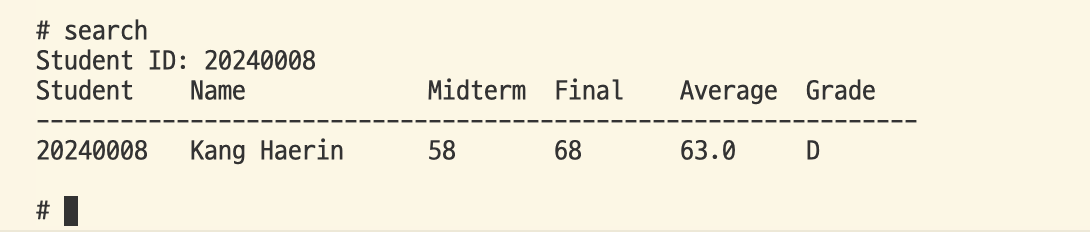
\includegraphics[width=\textwidth]{screenshots/3.png}
  \caption{실행 모습. search 명령어}
  \label{img:3}
\end{figure}
\begin{figure}
  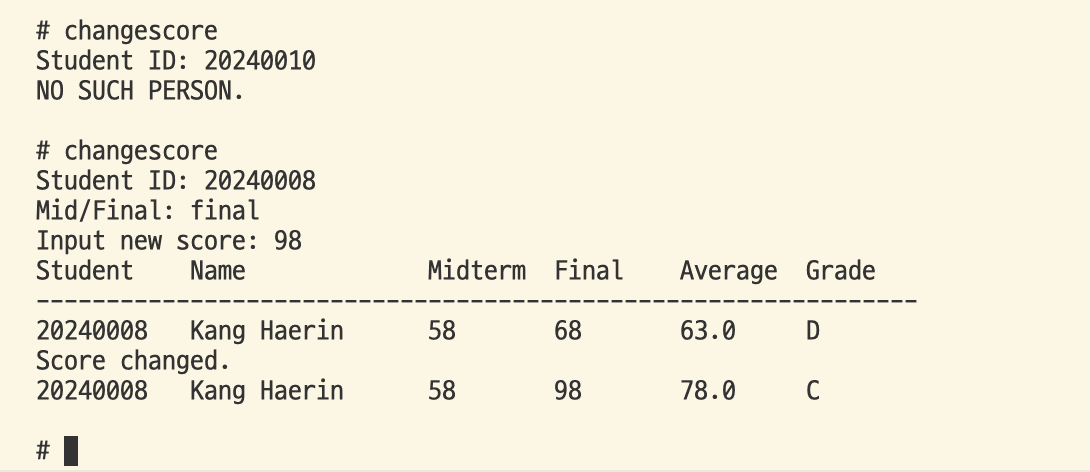
\includegraphics[width=\textwidth]{screenshots/4.png}
  \caption{실행 모습. changescore 명령어}
  \label{img:4}
\end{figure}
\begin{figure}
  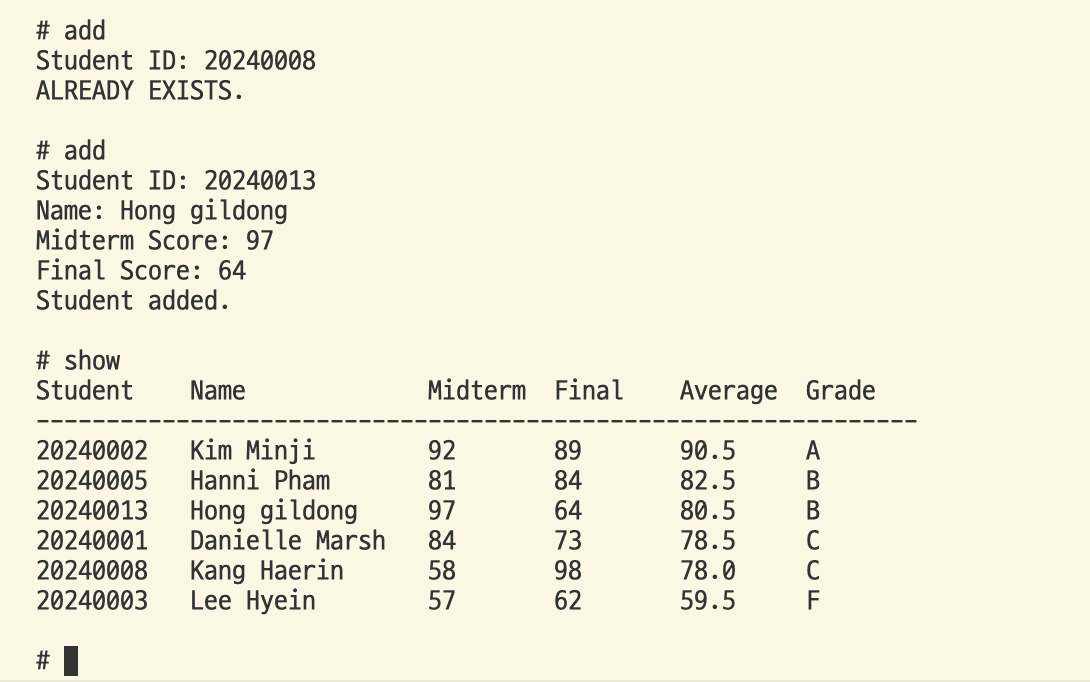
\includegraphics[width=\textwidth]{screenshots/5.png}
  \caption{실행 모습. add 명령어}
  \label{img:5}
\end{figure}
\begin{figure}
  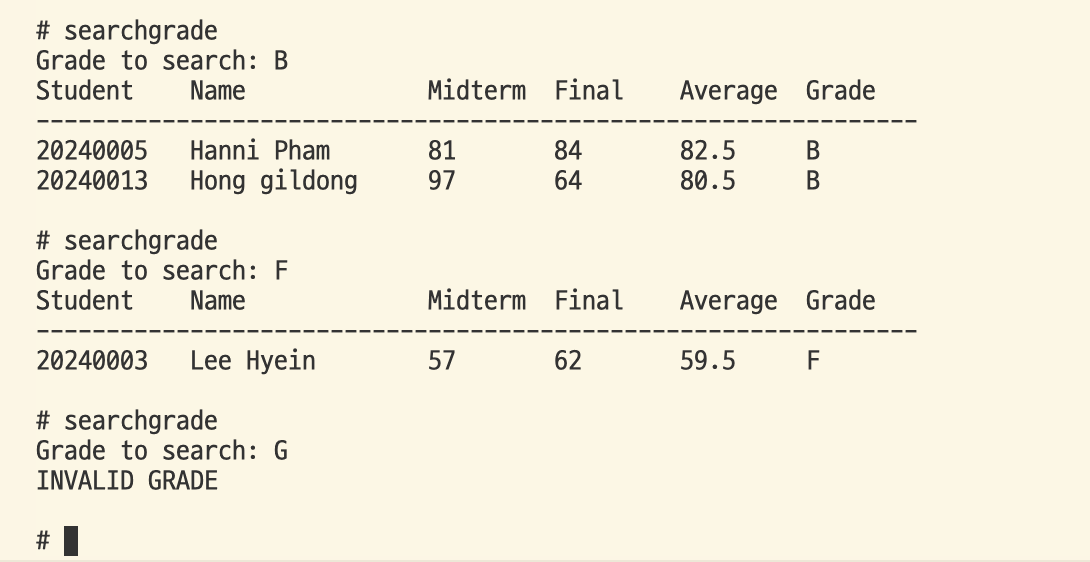
\includegraphics[width=\textwidth]{screenshots/6.png}
  \caption{실행 모습. searchgrade 명령어}
  \label{img:6}
\end{figure}
\begin{figure}
  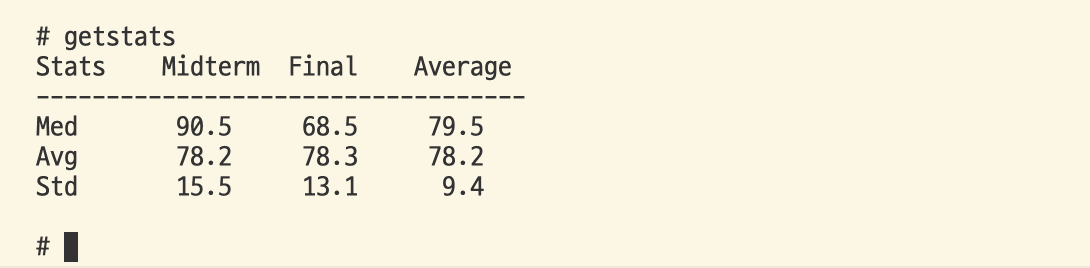
\includegraphics[width=\textwidth]{screenshots/7.png}
  \caption{실행 모습. getstats 명령어}
  \label{img:7}
\end{figure}
\begin{figure}
  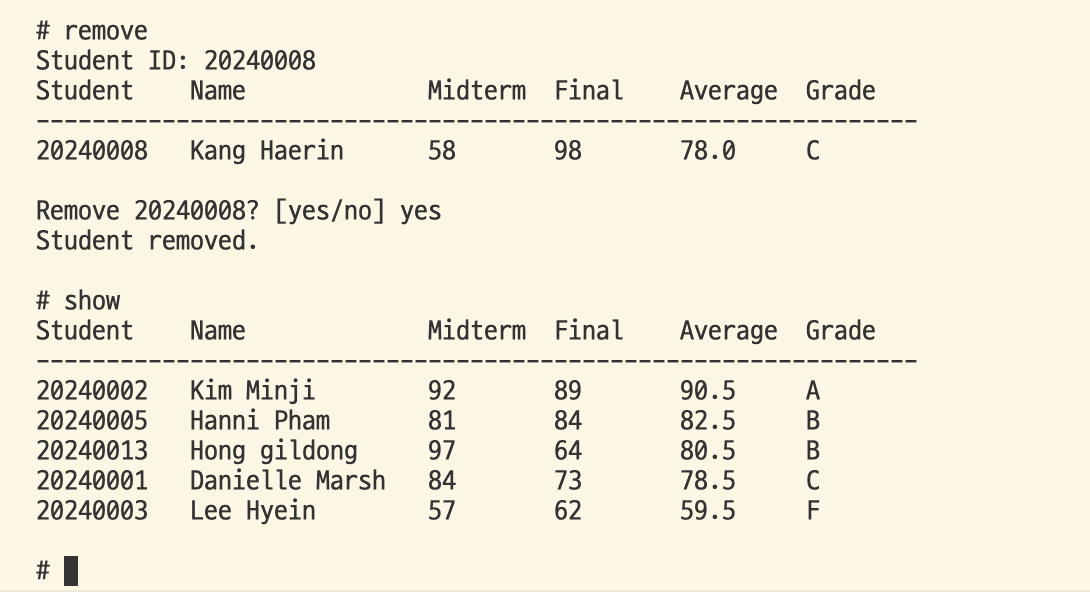
\includegraphics[width=\textwidth]{screenshots/8.png}
  \caption{실행 모습. remove 명령어}
  \label{img:8}
\end{figure}
\begin{figure}
  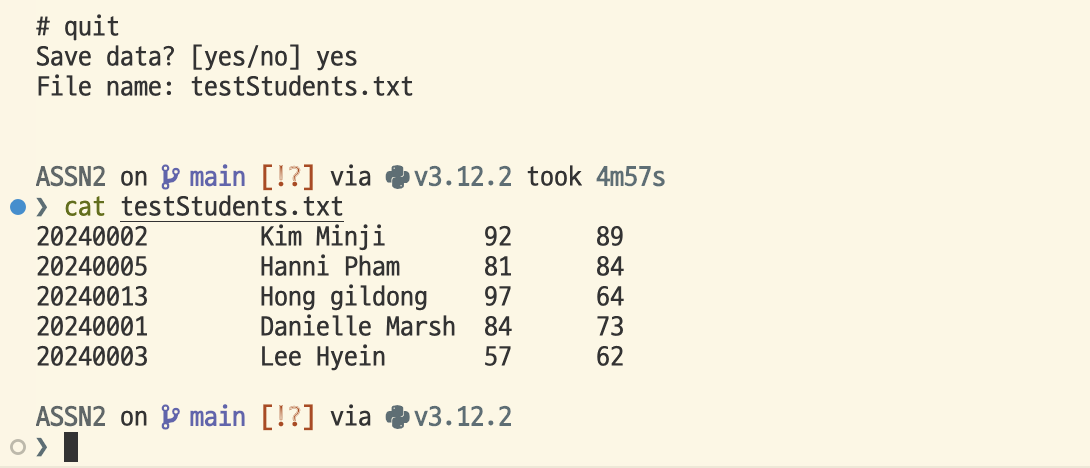
\includegraphics[width=\textwidth]{screenshots/9.png}
  \caption{실행 모습. quit 명령어}
  \label{img:9}
\end{figure}

\begin{itemize}
  \item 그림 \ref{img:1}\은 실행 직후의 모습으로
파일명으로 students.txt를 입력하였고, 해당 파일을 읽어 학생 목록을
출력하고 있다.
\item 
그림 \ref{img:2}\은 show 명령어 사용 모습으로, 모든 학생을 평균 점수로 정렬하여 목록으로 출력한다.
\item 
그림 \ref{img:3}\은 search 명령어 사용 모습으로, 원하는 학번을 입력하면 해당 학번에 해당하는 학생의 점수를 목록으로 출력한다.
\item 
그림 \ref{img:4}\은 changescore 명령어 사용 모습으로, 학번, 대상 시험(중간/기말), 점수를 입력하면 해당 학생의 점수를 수정한다. 존재하지 않는 학번을 입력하면 에러 메시지를 띄운다.
\item 
그림 \ref{img:5}\은 add 명령어 사용 모습으로, 학번, 이름, 점수를 입력받아 학생을 목록에 추가한다. 이미 존재하는 학번을 입력하면 에러 메시지가 나오며, 명령어 실행 후 show 명령어를 통해 학생이 정상적으로 추가되었음을 확인할 수 있다.
\item 
그림 \ref{img:6}\은 searchgrade 명령어 사용 모습으로, 원하는 학점을 입력하면 해당 학점을 가진 학생들을 목록으로 출력한다. 유효하지 않은 학번을 입력하면 에러 메시지가 출력된다.
\item 
그림 \ref{img:7}\은 getstats 명령어 사용 모습으로, 중간, 기말, 평균 점수에 대한 중앙값, 평균, 표준편차를 계산하여 표로 출력한다.
\item 
그림 \ref{img:8}\은 remove 명령어 사용 모습으로, 원하는 학번을 입력하면 해당 학번의 학생을 목록에서 삭제한다. 이후 show 명령어를 통해 실제로 삭제됨을 확인할 수 있다.
\item
그림 \ref{img:9}\은 quit 명령어 사용 모습으로, 데이터 저장 여부를 물어보며, 저장을 희망할 시 파일명을 입력받아 해당 파일에 학생 데이터를 저장하고 프로그램을 종료한다. cat 명령어로 실제로 파일에 잘 저장되었음을 보여주고 있다.
\end{itemize}

\section{토론}

\subsection{목록 출력}

목록을 출력할 일이 많았기 때문에 이를 별도 함수(print\_list와 관련 함수들)로 분리해 작성했다. 
처음에는 출력할 데이터를 담은 리스트만 인자로 받아 목록을 출력하는 함수 형태를 고안했으나, 
출력하는 목록은 2가지 종류(학생 목록, 통계값)가 있었기 때문에 헤더까지 인자로 받는 일반화된 함수 print\_list(header, body, padding)를 작성하고 이를 적절히 호출해 사용했다.
changescore에서 변경 전/후 비교 등 단순 목록이 아닌 경우에는 하위 함수(print\_list\_head, print\_list\_item)를 직접 호출하는 방식으로 구현했다.

\subsection{통계값 format 지정}

getstats 명령어 실행 시 통계값들을 계산해서 소숫점 첫째자리까지 출력해야했다.
보통 print 함수로 출력을 할 때 포멧을 변경하면 되지만,
이번 과제에서는 위에서 이야기했듯이 print\_list라는 일반화된 함수를 통해 출력을
하고 있었기 때문에 그렇게 할 수 없었다. 따라서 다른 방법을 고안하게 되었다.

처음에는 통계값을 계산하고 리스트에 저장할 때 포멧을 바꾸이 문자열로 저장하려고 했다.
하지만 평균은 이후 표준편차를 계산할 때 또 필요했기에 미리 문자열로 바꿀 수 없었다.
그래서 일단 계산값을 실수형으로 리스트에 저장하고, 마지막에 아래와 같이 순회를 돌며 모두 문자열로 바꾸는 방식으로 코드를 작성했다.

\begin{minted}[]{python3}
    for row in body:
        for i in range(1, 4):
            row[i] = f"{row[i]:5.1f}"
\end{minted}


\section{결론}

본 과제를 수행하며 이차원 리스트를 통해 데이터를 저장하고, 수정하고, 정렬하고, 출력하는 작업을 하며,
이차원 리스트를 더 자유자재로 다룰 수 있게 되었다.
파일 입출력하는 방법을 익힐 수 있었고, 다양한 사용자 정의 함수를 통해
효율적이고 구조화된 코드를 작성해보는 연습을 할 수 있었다.

\section{개선 방향}

대부분의 명령어 처리 함수에서 리스트가 비어있다면 "LIST IS EMPTY."라는 문구를
출력하는 부분이 등장한다. 이것이 중복되고 있으므로,
별도 로직으로 분리해서 중복을 제거하면 더 좋은 코드가 될 것 같다.

각 학생들의 평균과 학점을 계산해 리스트에 추가하는 코드 또한 여러 번 중복되고 있다.
이를 별도 함수로 분리하는 것도 좋을 것 같다.

\end{document}